% Graphic for TeX using PGF
% Title: /home/julien/master/projet/dessin-realite-augmentee/documents/uml/sequence_reseau.dia
% Creator: Dia v0.97.2
% CreationDate: Tue Apr 24 10:47:45 2012
% For: julien
% \usepackage{tikz}
% The following commands are not supported in PSTricks at present
% We define them conditionally, so when they are implemented,
% this pgf file will use them.
\ifx\du\undefined
  \newlength{\du}
\fi
\setlength{\du}{15\unitlength}
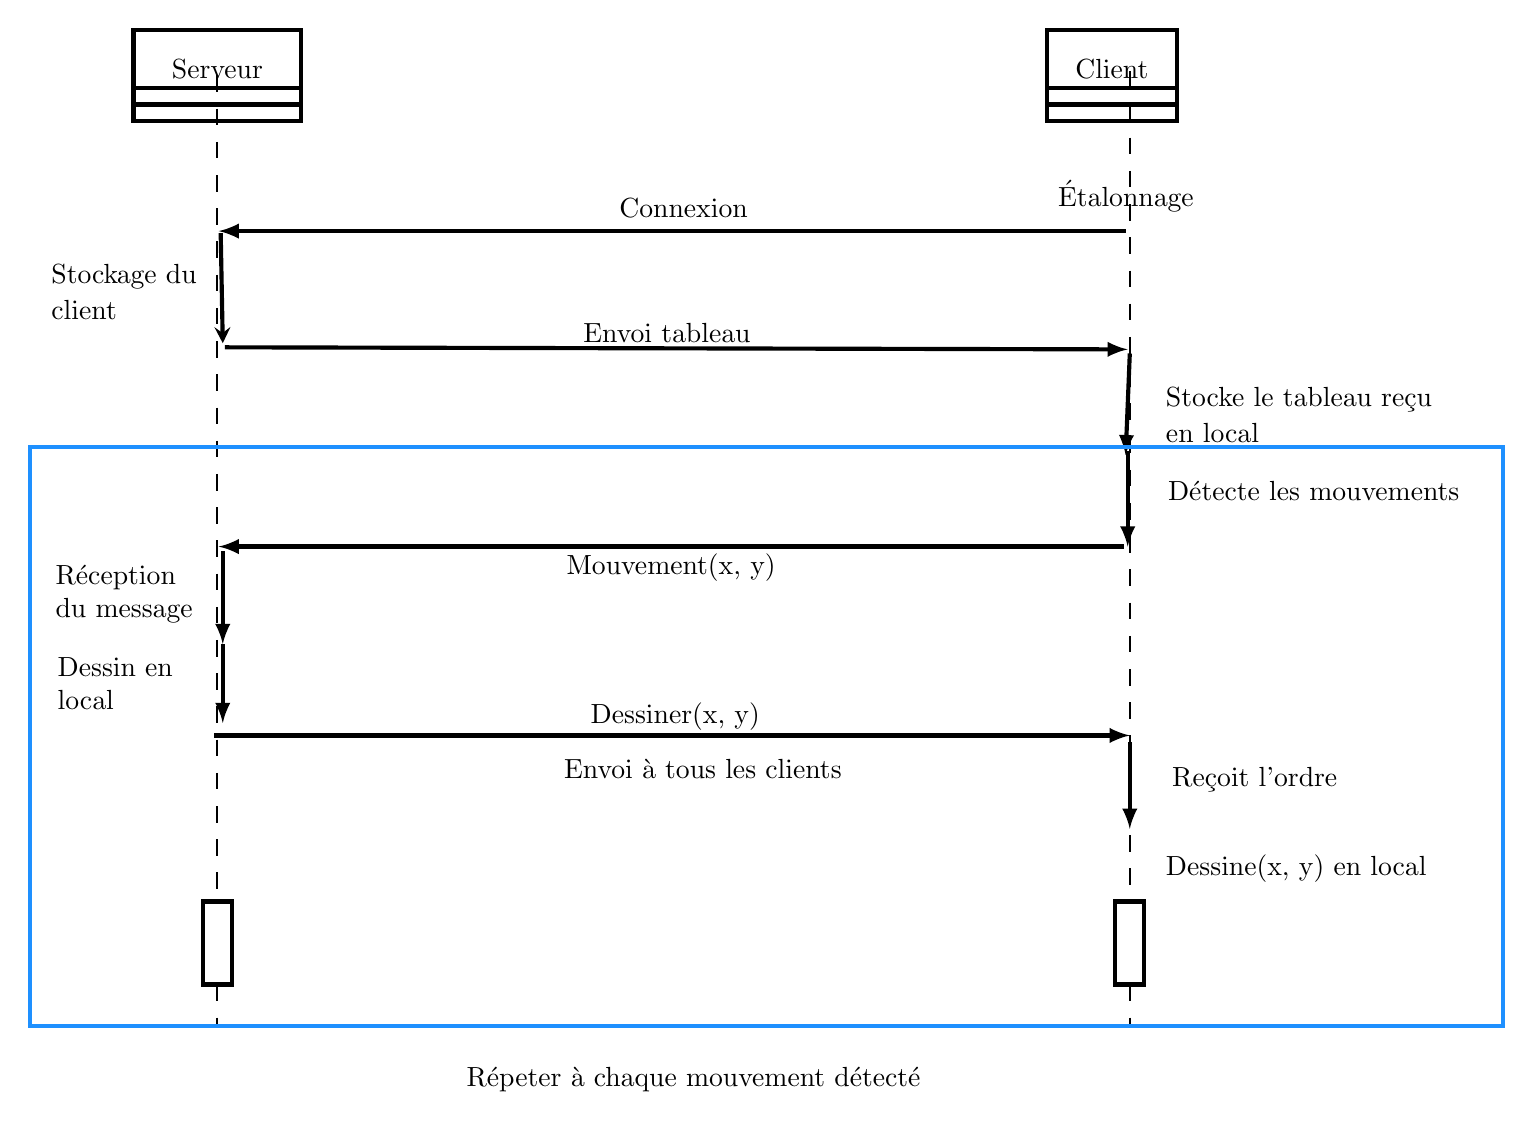
\begin{tikzpicture}
\pgftransformxscale{1.000000}
\pgftransformyscale{-1.000000}
\definecolor{dialinecolor}{rgb}{0.000000, 0.000000, 0.000000}
\pgfsetstrokecolor{dialinecolor}
\definecolor{dialinecolor}{rgb}{1.000000, 1.000000, 1.000000}
\pgfsetfillcolor{dialinecolor}
\pgfsetlinewidth{0.100000\du}
\pgfsetdash{}{0pt}
\definecolor{dialinecolor}{rgb}{1.000000, 1.000000, 1.000000}
\pgfsetfillcolor{dialinecolor}
\fill (5.000000\du,7.000000\du)--(5.000000\du,8.400000\du)--(9.042500\du,8.400000\du)--(9.042500\du,7.000000\du)--cycle;
\definecolor{dialinecolor}{rgb}{0.000000, 0.000000, 0.000000}
\pgfsetstrokecolor{dialinecolor}
\draw (5.000000\du,7.000000\du)--(5.000000\du,8.400000\du)--(9.042500\du,8.400000\du)--(9.042500\du,7.000000\du)--cycle;
% setfont left to latex
\definecolor{dialinecolor}{rgb}{0.000000, 0.000000, 0.000000}
\pgfsetstrokecolor{dialinecolor}
\node at (7.021250\du,7.950000\du){Serveur};
\definecolor{dialinecolor}{rgb}{1.000000, 1.000000, 1.000000}
\pgfsetfillcolor{dialinecolor}
\fill (5.000000\du,8.400000\du)--(5.000000\du,8.800000\du)--(9.042500\du,8.800000\du)--(9.042500\du,8.400000\du)--cycle;
\definecolor{dialinecolor}{rgb}{0.000000, 0.000000, 0.000000}
\pgfsetstrokecolor{dialinecolor}
\draw (5.000000\du,8.400000\du)--(5.000000\du,8.800000\du)--(9.042500\du,8.800000\du)--(9.042500\du,8.400000\du)--cycle;
\definecolor{dialinecolor}{rgb}{1.000000, 1.000000, 1.000000}
\pgfsetfillcolor{dialinecolor}
\fill (5.000000\du,8.800000\du)--(5.000000\du,9.200000\du)--(9.042500\du,9.200000\du)--(9.042500\du,8.800000\du)--cycle;
\definecolor{dialinecolor}{rgb}{0.000000, 0.000000, 0.000000}
\pgfsetstrokecolor{dialinecolor}
\draw (5.000000\du,8.800000\du)--(5.000000\du,9.200000\du)--(9.042500\du,9.200000\du)--(9.042500\du,8.800000\du)--cycle;
\pgfsetlinewidth{0.100000\du}
\pgfsetdash{}{0pt}
\definecolor{dialinecolor}{rgb}{1.000000, 1.000000, 1.000000}
\pgfsetfillcolor{dialinecolor}
\fill (27.000000\du,7.000000\du)--(27.000000\du,8.400000\du)--(30.132500\du,8.400000\du)--(30.132500\du,7.000000\du)--cycle;
\definecolor{dialinecolor}{rgb}{0.000000, 0.000000, 0.000000}
\pgfsetstrokecolor{dialinecolor}
\draw (27.000000\du,7.000000\du)--(27.000000\du,8.400000\du)--(30.132500\du,8.400000\du)--(30.132500\du,7.000000\du)--cycle;
% setfont left to latex
\definecolor{dialinecolor}{rgb}{0.000000, 0.000000, 0.000000}
\pgfsetstrokecolor{dialinecolor}
\node at (28.566250\du,7.950000\du){Client};
\definecolor{dialinecolor}{rgb}{1.000000, 1.000000, 1.000000}
\pgfsetfillcolor{dialinecolor}
\fill (27.000000\du,8.400000\du)--(27.000000\du,8.800000\du)--(30.132500\du,8.800000\du)--(30.132500\du,8.400000\du)--cycle;
\definecolor{dialinecolor}{rgb}{0.000000, 0.000000, 0.000000}
\pgfsetstrokecolor{dialinecolor}
\draw (27.000000\du,8.400000\du)--(27.000000\du,8.800000\du)--(30.132500\du,8.800000\du)--(30.132500\du,8.400000\du)--cycle;
\definecolor{dialinecolor}{rgb}{1.000000, 1.000000, 1.000000}
\pgfsetfillcolor{dialinecolor}
\fill (27.000000\du,8.800000\du)--(27.000000\du,9.200000\du)--(30.132500\du,9.200000\du)--(30.132500\du,8.800000\du)--cycle;
\definecolor{dialinecolor}{rgb}{0.000000, 0.000000, 0.000000}
\pgfsetstrokecolor{dialinecolor}
\draw (27.000000\du,8.800000\du)--(27.000000\du,9.200000\du)--(30.132500\du,9.200000\du)--(30.132500\du,8.800000\du)--cycle;
\pgfsetlinewidth{0.050000\du}
\pgfsetdash{}{0pt}
\pgfsetdash{{0.400000\du}{0.400000\du}}{0\du}
\definecolor{dialinecolor}{rgb}{0.000000, 0.000000, 0.000000}
\pgfsetstrokecolor{dialinecolor}
\draw (29.000000\du,8.000000\du)--(29.000000\du,28.000000\du);
\definecolor{dialinecolor}{rgb}{0.000000, 0.000000, 0.000000}
\pgfsetstrokecolor{dialinecolor}
\draw (29.000000\du,30.000000\du)--(29.000000\du,31.000000\du);
\pgfsetlinewidth{0.100000\du}
\pgfsetdash{}{0pt}
\definecolor{dialinecolor}{rgb}{1.000000, 1.000000, 1.000000}
\pgfsetfillcolor{dialinecolor}
\fill (28.650000\du,28.000000\du)--(28.650000\du,30.000000\du)--(29.350000\du,30.000000\du)--(29.350000\du,28.000000\du)--cycle;
\definecolor{dialinecolor}{rgb}{0.000000, 0.000000, 0.000000}
\pgfsetstrokecolor{dialinecolor}
\draw (28.650000\du,28.000000\du)--(28.650000\du,30.000000\du)--(29.350000\du,30.000000\du)--(29.350000\du,28.000000\du)--cycle;
\pgfsetlinewidth{0.050000\du}
\pgfsetdash{}{0pt}
\pgfsetdash{{0.400000\du}{0.400000\du}}{0\du}
\definecolor{dialinecolor}{rgb}{0.000000, 0.000000, 0.000000}
\pgfsetstrokecolor{dialinecolor}
\draw (7.021250\du,8.100000\du)--(7.021250\du,28.000000\du);
\definecolor{dialinecolor}{rgb}{0.000000, 0.000000, 0.000000}
\pgfsetstrokecolor{dialinecolor}
\draw (7.021250\du,30.000000\du)--(7.021250\du,31.000000\du);
\pgfsetlinewidth{0.100000\du}
\pgfsetdash{}{0pt}
\definecolor{dialinecolor}{rgb}{1.000000, 1.000000, 1.000000}
\pgfsetfillcolor{dialinecolor}
\fill (6.671250\du,28.000000\du)--(6.671250\du,30.000000\du)--(7.371250\du,30.000000\du)--(7.371250\du,28.000000\du)--cycle;
\definecolor{dialinecolor}{rgb}{0.000000, 0.000000, 0.000000}
\pgfsetstrokecolor{dialinecolor}
\draw (6.671250\du,28.000000\du)--(6.671250\du,30.000000\du)--(7.371250\du,30.000000\du)--(7.371250\du,28.000000\du)--cycle;
\pgfsetlinewidth{0.100000\du}
\pgfsetbuttcap
\pgfsetdash{}{0pt}
{
\definecolor{dialinecolor}{rgb}{0.000000, 0.000000, 0.000000}
\pgfsetfillcolor{dialinecolor}
% was here!!!
\pgfsetarrowsstart{latex}
\definecolor{dialinecolor}{rgb}{0.000000, 0.000000, 0.000000}
\pgfsetstrokecolor{dialinecolor}
\draw (7.050000\du,11.850000\du)--(28.900000\du,11.850000\du);
}
% setfont left to latex
\definecolor{dialinecolor}{rgb}{0.000000, 0.000000, 0.000000}
\pgfsetstrokecolor{dialinecolor}
\node at (18.250000\du,11.300000\du){Connexion};
\pgfsetlinewidth{0.100000\du}
\pgfsetdash{}{0pt}
\pgfsetdash{}{0pt}
\pgfsetbuttcap
{
\definecolor{dialinecolor}{rgb}{0.000000, 0.000000, 0.000000}
\pgfsetfillcolor{dialinecolor}
% was here!!!
\pgfsetarrowsend{stealth}
\definecolor{dialinecolor}{rgb}{0.000000, 0.000000, 0.000000}
\pgfsetstrokecolor{dialinecolor}
\draw (7.100000\du,11.900000\du)--(7.150000\du,14.550000\du);
}
\pgfsetlinewidth{0.100000\du}
\pgfsetbuttcap
\pgfsetdash{}{0pt}
{
\definecolor{dialinecolor}{rgb}{0.000000, 0.000000, 0.000000}
\pgfsetfillcolor{dialinecolor}
% was here!!!
\pgfsetarrowsstart{latex}
\definecolor{dialinecolor}{rgb}{0.000000, 0.000000, 0.000000}
\pgfsetstrokecolor{dialinecolor}
\draw (28.950000\du,14.700000\du)--(7.200000\du,14.650000\du);
}
% setfont left to latex
\definecolor{dialinecolor}{rgb}{0.000000, 0.000000, 0.000000}
\pgfsetstrokecolor{dialinecolor}
\node at (17.850000\du,14.300000\du){Envoi tableau};
% setfont left to latex
\definecolor{dialinecolor}{rgb}{0.000000, 0.000000, 0.000000}
\pgfsetstrokecolor{dialinecolor}
\node[anchor=west] at (27.000000\du,11.000000\du){Étalonnage};
% setfont left to latex
\definecolor{dialinecolor}{rgb}{0.000000, 0.000000, 0.000000}
\pgfsetstrokecolor{dialinecolor}
\node[anchor=west] at (2.750000\du,12.950000\du){Stockage du };
% setfont left to latex
\definecolor{dialinecolor}{rgb}{0.000000, 0.000000, 0.000000}
\pgfsetstrokecolor{dialinecolor}
\node[anchor=west] at (2.750000\du,13.750000\du){client};
\pgfsetlinewidth{0.100000\du}
\pgfsetbuttcap
\pgfsetdash{}{0pt}
{
\definecolor{dialinecolor}{rgb}{0.000000, 0.000000, 0.000000}
\pgfsetfillcolor{dialinecolor}
% was here!!!
\pgfsetarrowsstart{latex}
\definecolor{dialinecolor}{rgb}{0.000000, 0.000000, 0.000000}
\pgfsetstrokecolor{dialinecolor}
\draw (28.900000\du,17.250000\du)--(29.000000\du,14.800000\du);
}
% setfont left to latex
% setfont left to latex
\definecolor{dialinecolor}{rgb}{0.000000, 0.000000, 0.000000}
\pgfsetstrokecolor{dialinecolor}
\node[anchor=west] at (29.600000\du,15.900000\du){Stocke le tableau reçu};
% setfont left to latex
\definecolor{dialinecolor}{rgb}{0.000000, 0.000000, 0.000000}
\pgfsetstrokecolor{dialinecolor}
\node[anchor=west] at (29.600000\du,16.700000\du){en local};
\pgfsetlinewidth{0.100000\du}
\pgfsetbuttcap
\pgfsetdash{}{0pt}
{
\definecolor{dialinecolor}{rgb}{0.000000, 0.000000, 0.000000}
\pgfsetfillcolor{dialinecolor}
% was here!!!
\pgfsetarrowsstart{latex}
\definecolor{dialinecolor}{rgb}{0.000000, 0.000000, 0.000000}
\pgfsetstrokecolor{dialinecolor}
\draw (7.050000\du,19.450000\du)--(28.850000\du,19.450000\du);
}
% setfont left to latex
\definecolor{dialinecolor}{rgb}{0.000000, 0.000000, 0.000000}
\pgfsetstrokecolor{dialinecolor}
\node at (17.950000\du,19.950000\du){Mouvement(x, y)};
% setfont left to latex
\definecolor{dialinecolor}{rgb}{0.000000, 0.000000, 0.000000}
\pgfsetstrokecolor{dialinecolor}
\node[anchor=west] at (2.850000\du,20.200000\du){Réception };
% setfont left to latex
\definecolor{dialinecolor}{rgb}{0.000000, 0.000000, 0.000000}
\pgfsetstrokecolor{dialinecolor}
\node[anchor=west] at (2.850000\du,21.000000\du){du message};
% setfont left to latex
\definecolor{dialinecolor}{rgb}{0.000000, 0.000000, 0.000000}
\pgfsetstrokecolor{dialinecolor}
\node[anchor=west] at (2.900000\du,22.350000\du){Dessin en};
% setfont left to latex
\definecolor{dialinecolor}{rgb}{0.000000, 0.000000, 0.000000}
\pgfsetstrokecolor{dialinecolor}
\node[anchor=west] at (2.900000\du,23.150000\du){local};
\pgfsetlinewidth{0.100000\du}
\pgfsetbuttcap
\pgfsetdash{}{0pt}
{
\definecolor{dialinecolor}{rgb}{0.000000, 0.000000, 0.000000}
\pgfsetfillcolor{dialinecolor}
% was here!!!
\pgfsetarrowsstart{latex}
\definecolor{dialinecolor}{rgb}{0.000000, 0.000000, 0.000000}
\pgfsetstrokecolor{dialinecolor}
\draw (7.150000\du,21.800000\du)--(7.150000\du,19.550000\du);
}
% setfont left to latex
\pgfsetlinewidth{0.100000\du}
\pgfsetbuttcap
\pgfsetdash{}{0pt}
{
\definecolor{dialinecolor}{rgb}{0.000000, 0.000000, 0.000000}
\pgfsetfillcolor{dialinecolor}
% was here!!!
\pgfsetarrowsstart{latex}
\definecolor{dialinecolor}{rgb}{0.000000, 0.000000, 0.000000}
\pgfsetstrokecolor{dialinecolor}
\draw (7.150000\du,23.700000\du)--(7.150000\du,21.800000\du);
}
% setfont left to latex
\pgfsetlinewidth{0.100000\du}
\pgfsetbuttcap
\pgfsetdash{}{0pt}
{
\definecolor{dialinecolor}{rgb}{0.000000, 0.000000, 0.000000}
\pgfsetfillcolor{dialinecolor}
% was here!!!
\pgfsetarrowsstart{latex}
\definecolor{dialinecolor}{rgb}{0.000000, 0.000000, 0.000000}
\pgfsetstrokecolor{dialinecolor}
\draw (28.950000\du,19.450000\du)--(28.950000\du,17.150000\du);
}
% setfont left to latex
% setfont left to latex
\definecolor{dialinecolor}{rgb}{0.000000, 0.000000, 0.000000}
\pgfsetstrokecolor{dialinecolor}
\node[anchor=west] at (29.650000\du,18.100000\du){Détecte les mouvements};
\pgfsetlinewidth{0.100000\du}
\pgfsetbuttcap
\pgfsetdash{}{0pt}
{
\definecolor{dialinecolor}{rgb}{0.000000, 0.000000, 0.000000}
\pgfsetfillcolor{dialinecolor}
% was here!!!
\pgfsetarrowsstart{latex}
\definecolor{dialinecolor}{rgb}{0.000000, 0.000000, 0.000000}
\pgfsetstrokecolor{dialinecolor}
\draw (29.000000\du,24.000000\du)--(6.950000\du,24.000000\du);
}
% setfont left to latex
\definecolor{dialinecolor}{rgb}{0.000000, 0.000000, 0.000000}
\pgfsetstrokecolor{dialinecolor}
\node at (18.050000\du,23.550000\du){Dessiner(x, y)};
% setfont left to latex
\definecolor{dialinecolor}{rgb}{0.000000, 0.000000, 0.000000}
\pgfsetstrokecolor{dialinecolor}
\node[anchor=west] at (15.100000\du,24.800000\du){Envoi à tous les clients};
\pgfsetlinewidth{0.100000\du}
\pgfsetbuttcap
\pgfsetdash{}{0pt}
{
\definecolor{dialinecolor}{rgb}{0.000000, 0.000000, 0.000000}
\pgfsetfillcolor{dialinecolor}
% was here!!!
\pgfsetarrowsstart{latex}
\definecolor{dialinecolor}{rgb}{0.000000, 0.000000, 0.000000}
\pgfsetstrokecolor{dialinecolor}
\draw (29.000000\du,26.250000\du)--(29.000000\du,24.150000\du);
}
% setfont left to latex
% setfont left to latex
\definecolor{dialinecolor}{rgb}{0.000000, 0.000000, 0.000000}
\pgfsetstrokecolor{dialinecolor}
\node[anchor=west] at (29.750000\du,25.050000\du){Reçoit l'ordre};
% setfont left to latex
\definecolor{dialinecolor}{rgb}{0.000000, 0.000000, 0.000000}
\pgfsetstrokecolor{dialinecolor}
\node[anchor=west] at (29.600000\du,27.200000\du){Dessine(x, y) en local};
\pgfsetlinewidth{0.100000\du}
\pgfsetdash{}{0pt}
\pgfsetdash{}{0pt}
\pgfsetmiterjoin
\definecolor{dialinecolor}{rgb}{0.117647, 0.564706, 1.000000}
\pgfsetstrokecolor{dialinecolor}
\draw (2.500000\du,17.050000\du)--(2.500000\du,31.000000\du)--(38.000000\du,31.000000\du)--(38.000000\du,17.050000\du)--cycle;
% setfont left to latex
\definecolor{dialinecolor}{rgb}{0.117647, 0.564706, 1.000000}
\pgfsetstrokecolor{dialinecolor}
\node[anchor=west] at (12.750000\du,32.300000\du){Répeter à chaque mouvement détecté};
\end{tikzpicture}
